\documentclass[12pt,fleqn]{article}

\usepackage[utf8]{inputenc}
\usepackage[T2A]{fontenc}
\usepackage{amssymb,amsmath,mathrsfs,amsthm}
\usepackage[russian]{babel}
\usepackage[pdftex]{graphicx}
\usepackage{multirow}
\usepackage[footnotesize]{caption2}
\usepackage{indentfirst}
\usepackage[colorlinks, unicode]{hyperref}


%\usepackage[ruled,section]{algorithm}
%\usepackage[noend]{algorithmic}
%\usepackage[all]{xy}

% Параметры страницы
\textheight=24cm % высота текста
\textwidth=16cm % ширина текста
\oddsidemargin=0pt % отступ от левого края
\topmargin=-2.5cm % отступ от верхнего края
\parindent=24pt % абзацный отступ
\parskip=0pt % интервал между абзацам
\tolerance=2000 % терпимость к "жидким" строкам
\flushbottom % выравнивание высоты страниц
%\def\baselinestretch{1.5}
\setcounter{secnumdepth}{0}
\renewcommand{\baselinestretch}{1.1}

\newcommand{\norm}{\mathop{\rm norm}\limits}
\newcommand{\real}{\mathbb{R}}

\newcommand{\ex}{\mathbb{E}}
\newcommand{\diag}{\mathrm{diag}}
\newcommand{\intset}{\mathrm{int}}
\newcommand{\softmax}{\mathop{\rm softmax}\limits}
\newcommand{\lossfunc}{\mathcal{L}'}
\newcommand{\elbo}{\mathcal{L}}
\newcommand{\normal}[3]{\mathcal{N}(#1 | #2, #3)}
\newcommand{\dd}[2]{\frac{\partial#1}{\partial#2}}
\newcommand{\kl}[2]{\mathop{KL}(#1 \parallel #2)}
\newcommand{\nm}{\mathcal{N}}
\newcommand{\sle}{\; \Rightarrow \;}
\newcommand{\indpos}{\mathbf{I}_{d_k}^{+}[i, j]}
\newcommand{\indneg}{\mathbf{I}_{d_k}^{-}[i, j]}

\usepackage{pgfplots}

%my settings
\graphicspath{{../figures/}}

\title{Исследование работы алгоритма KNearestNeighbors 

на примере датасета MNIST}

\author{Тыцкий Владислав}
\date{Октябрь 2020}

\begin{document}

\maketitle

\section{Введение}
Требуется решить задачу классификации с помощью метрического метода KNearestNeighbors(метод К ближайших соседей)
 на примере известного датасета  MNIST.
 
 MNIST - база данных рукописных цифр. Каждая цифра представляется в виде  черно-белого изображения  $28\times28$ пикселей,
  что эквивалентно вектору 
 $x \in \mathbb{R}^{784}$. Датасет содержит 70000 размеченных цифр. В данном исследовании мы будем использовать 
 обучающую выборку размера 60000, а тестовую соответсвенно 10000.
 \footnote{В некоторых частях исследования будет использоваться уменьшенная выборка т.к. вычислительная 
 машина Тыцкого В.И. тяжело справляется с такой нагрузкой. Во всех случаях, где не оговаривается иное,
 будет использоваться полная выборка}

\section{Задание №1}
Сравним различные алгоритмы нахождения ближайших соседей --- brute, kd\_tree, ball\_tree и my\_own. 

my\_own --- самописная реализация, которая вычисляет полную матрицу расстояний $D^{T \times N}$, где T -- размер 
тестовой выборки, N -- размер обучающей выборки.

brute, kd\_tree, ball\_tree --- реализации поиска соседей из библиотеки sklearn.
\subsection{Сравнение скорости работы}
Так как описанные выше методы нахождения соседей являются детерминированными (100\% точными), то главным критерием 
выбора одного из них для дальнеших исследований будет служить скорость работы.
В случае MNIST важно знать как хорошо ведут себя алгоритмы в пространстве большой размерности $\mathbb{R}^{784}$. 

Для экспериментов были выбраны подпространства размерности 10, 50 , 100.
В качестве меры расстояния возьмем евклидову метрику.
\newpage
На графике (Рис.\ref{pic1}) представлены результаты вычисления ближайших соседей для тестовой выборки размера 3000 и 10000
для обучающей выборки. 
%\setlength{\textfloatsep}{40pt}
\begin{figure}
    \centering
    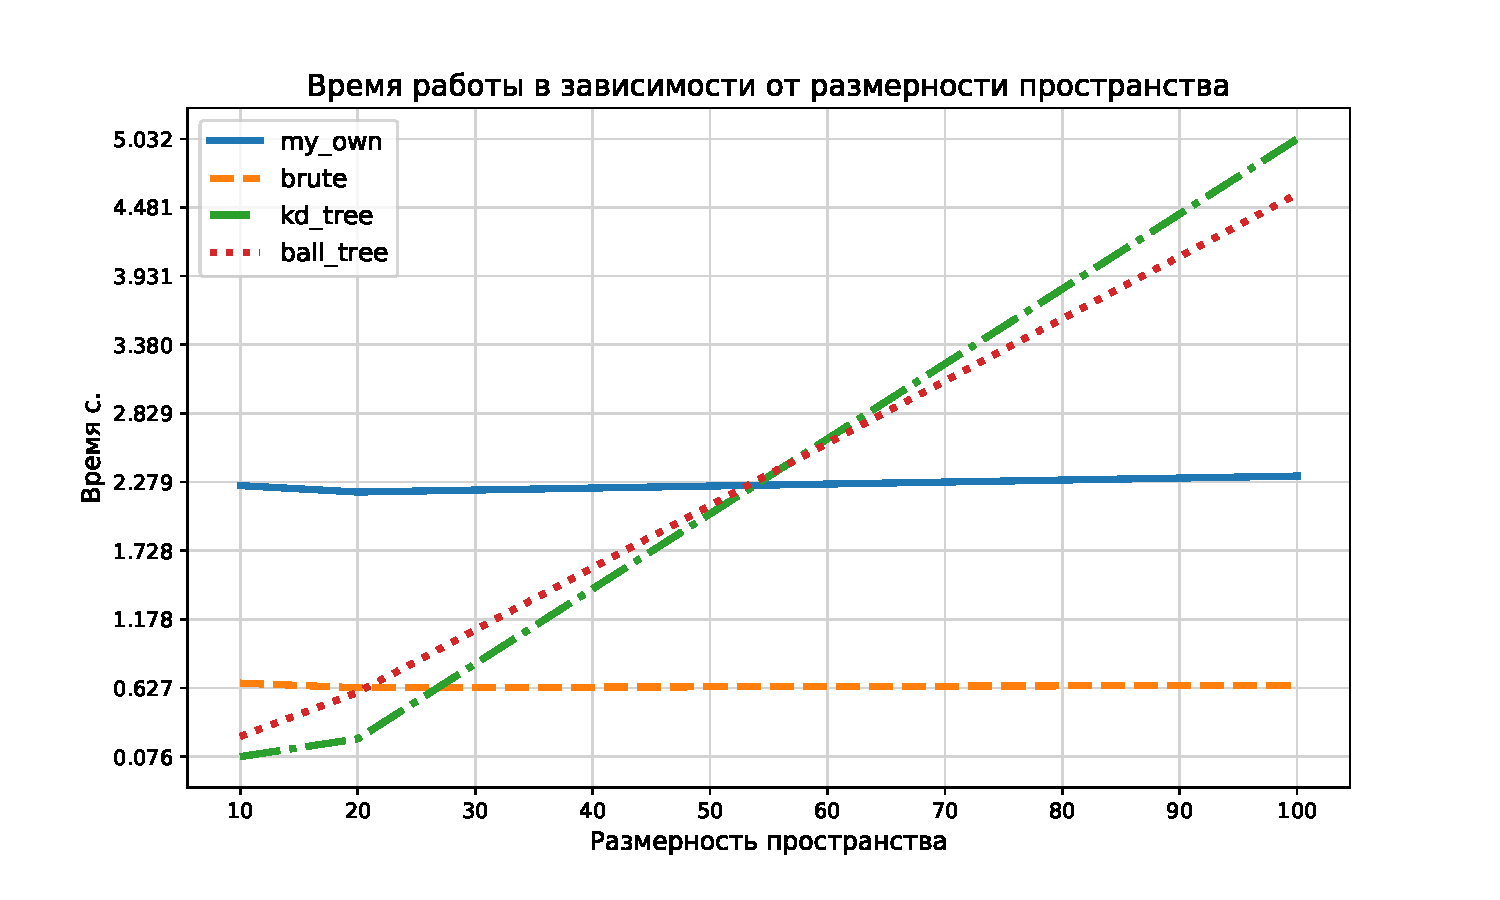
\includegraphics[width=15cm]{task1.pdf} 
    \caption{}
    \label{pic1}
\end{figure}

Из графика время работы kd\_tree и ball\_tree с ростом размерности пространства увеличивается линейно.
Это связано с принципами работы алгоритма и так явлением называемым ``Проклятие размерности''.
Brute и my\_own имеют практически константое время работы алгортима, потому что основаны на простом построении матрицы 
расстояний,  вычисление нормы разности $||x_i-x_j||$  по сравнению с построением матрицы имеет
незначительное количество операций. 

Далее везде будем использовать либо brute, либо my\_own 
\footnote{Кроме евклидовой метрики нам понадобится косинусное расстояние---
$cos(x, y)=1- \frac{(x, y)}{||x||_2||y||_2}$.
Sklearn метод, реализующих поиск соседей не поддерживает косинусное расстояние,
поэтому часто будем использовать метод my\_own, у которого есть поддержка этого расстояния.}

\section{Задание №2/3}
Требуется по кросс-валидации с тремя фолдами оценить точность и время работы в зависимости от следующих
факторов:
\begin{enumerate}
    \item k от 1 до 10 (только точность)
    \item евклидова или косинусная метрика
    \item используются ли веса или нет (только точность)
    \footnote{$w_k=\frac{1}{\rho(X,X_k)+10^{-5}}$, где w\_k вес K-ого ближайшего соседа X\_k для X}
\end{enumerate}
Кросс-валидация проводилась на обучающей выборке размером 60000
\newpage

\begin{figure}
    \centering
    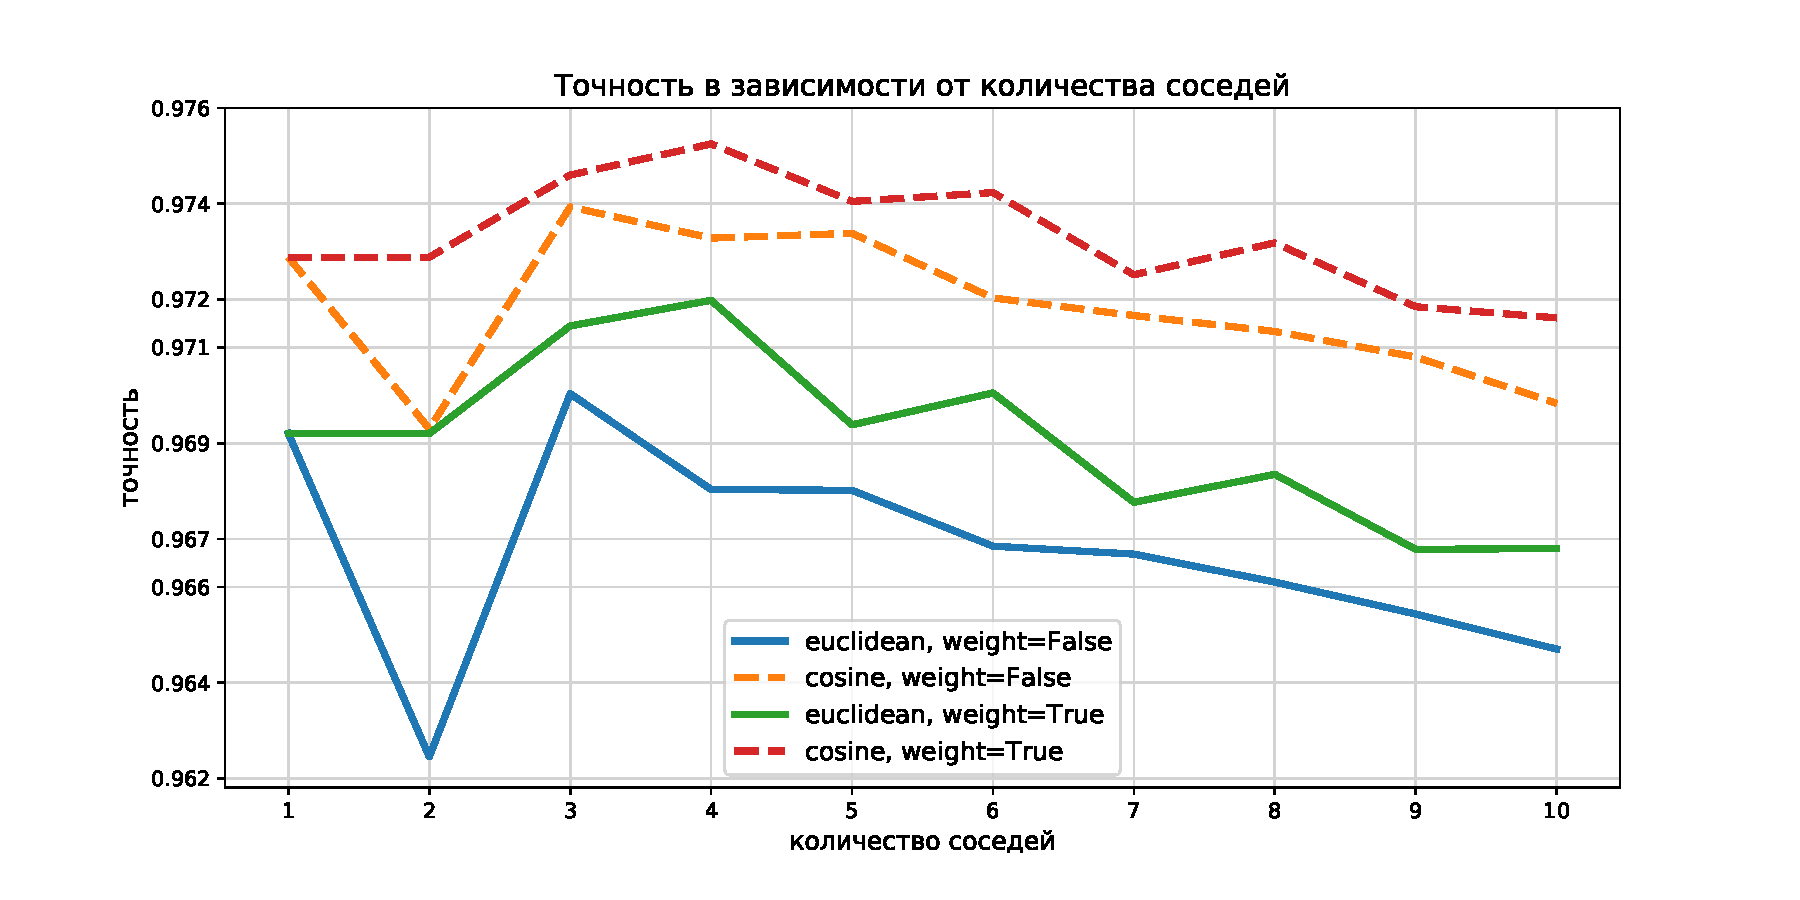
\includegraphics[width=17cm]{task2.pdf}
    \caption{}
    \label{pic2}
\end{figure}

На графике (Рис.\ref{pic2}) представлены результаты вычисления качества в зависимости от
вышеперечисленных параметров


\begin{itemize}
    \item Косинусное расстояние(с весами и без) лучше евклидова для любых k.
    \item Использование весов улучшает качество для любых $k$.
    \item Качество постепенно падает у всех алгоритмов, если $k>4$
    \item Лучшим оказался алгоритм с $k=4$ использующий косинусное расстояние и веса.
    \textbf{Его точность: 0.975}
\end{itemize}

Интересно, что без весов лучшее качество достигается при $k=3$, а с весами  при $k=4$. 
Это говорит о том,что веса в некотором смысле регуляризуют модель --- она
использует информацию от большего числа соседей, но не ``доверяет'' слишком далеким объектам.

\newpage
\subsubsection{Скорость работы}
Посмотрим влияет ли метрика на скорость работы алгортима. В обоих используется my\_own.
Размер обучающей выборки 10000.

\begin{table}[htb]
    \centering
    \begin{tabular}{|c|c|c|c|c|}
    \hline
    \multirow{2}{*}{\textbf{test size}} & \multicolumn{2}{c|}{\textbf{euclidean}} & \multicolumn{2}{c|}{\textbf{cosine}} \\ \cline{2-5} 
                                        & mean(sec)           & std(sec)          & mean(sec)         & std(sec)         \\ \hline
    \textbf{1000}                       & 0.917               & 0.015             & 0.900             & 0.001            \\ \hline
    \textbf{2000}                       & 1.710               & 0.027             & 1.796             & 0.113            \\ \hline
    \textbf{3000}                       & 2.547               & 0.021             & 2.608             & 0.025           \\ \hline
    \end{tabular}
    \caption{Сравнение скорости работы в зависимости от метрики}
\end{table}

Можно сделать вывод, что метрика не влияет на скорость работы алгоритма. Это вполне логично ---
 обе реалзиции работают с асимптотикой $\Theta(n^{2.3727})$ (Алгоритм Копперсмита -- Винограда)
\newpage
\section{Задание №4}
Применим лучший алгоритм (cosine, k=5) для тестовой выборки размером 10000. 
\textbf{Точность на тесте: 0.9771}

\subsection{Сравнение с лучшими алгоритмами}

Рассмотрим таблицу (Таблица \ref{table2}) лучших алгоритмов для датасета MNIST.
\begin{table}[htb]
    \centering
    \begin{tabular}{|l|l|l|}
    \hline
    Type                                          & Preprocessing                       & Error rate (\%) \\ \hline
    Convolutional neural network                  & Data augmentation                   & 0.17            \\ \hline
    Random Multimodel Deep Learning (RMDL)        & None                                & 0.18            \\ \hline
    Convolutional neural network                  & Expansion of the train data      & 0.21            \\ \hline
    Convolutional neural network                  & Width normalizations                & 0.23            \\ \hline
    Convolutional neural network                  & Expansion of the train data      & 0.27            \\ \hline
    Convolutional neural network (CNN)            & Expansion of the train data      & 0.31            \\ \hline
    Deep neural network                           & None                                & 0.35            \\ \hline
    K-Nearest Neighbors                           & Shiftable edges                     & 0.52            \\ \hline
    Support-vector machine (SVM)                  & Deskewing                           & 0.56            \\ \hline
    Deep neural network                           & None                                & 0.7             \\ \hline
    Boosted Stumps                                & Haar features                       & 0.87            \\ \hline
    Deep neural network (DNN)                     & None                                & 1.6             \\ \hline
    \textbf{K-Nearest Neighbors (my realisation)} & \textbf{None}                       & \textbf{2.3}    \\ \hline
    Random Forest                                 & Statistical pixel importance        & 2.8             \\ \hline
    Non-linear classifier                         & None                                & 3.3             \\ \hline
    Linear classifier                             & Deskewing                           & 7.6             \\ \hline
    \end{tabular}
    \caption{Сравнение с лучшими алгоритмами}
    \label{table2}
\end{table}

Даже на бейзлайне мы получаем неплохие результаты. С accuracy 0.948 в таблице присутствует другой
алгоритм KNN \cite{deformationmodels}


\subsection{Ошибки алгоритма}

Интересно взглянуть на каких именно объектах наша модель ошибалась. Для этого построим 
матрицу ошибок(confusion matrix) (Рис.\ref{pic3}. Значения на диагонали убраны, в данном случае они нам неинтересны.
\newpage
\begin{figure}
    \centering
    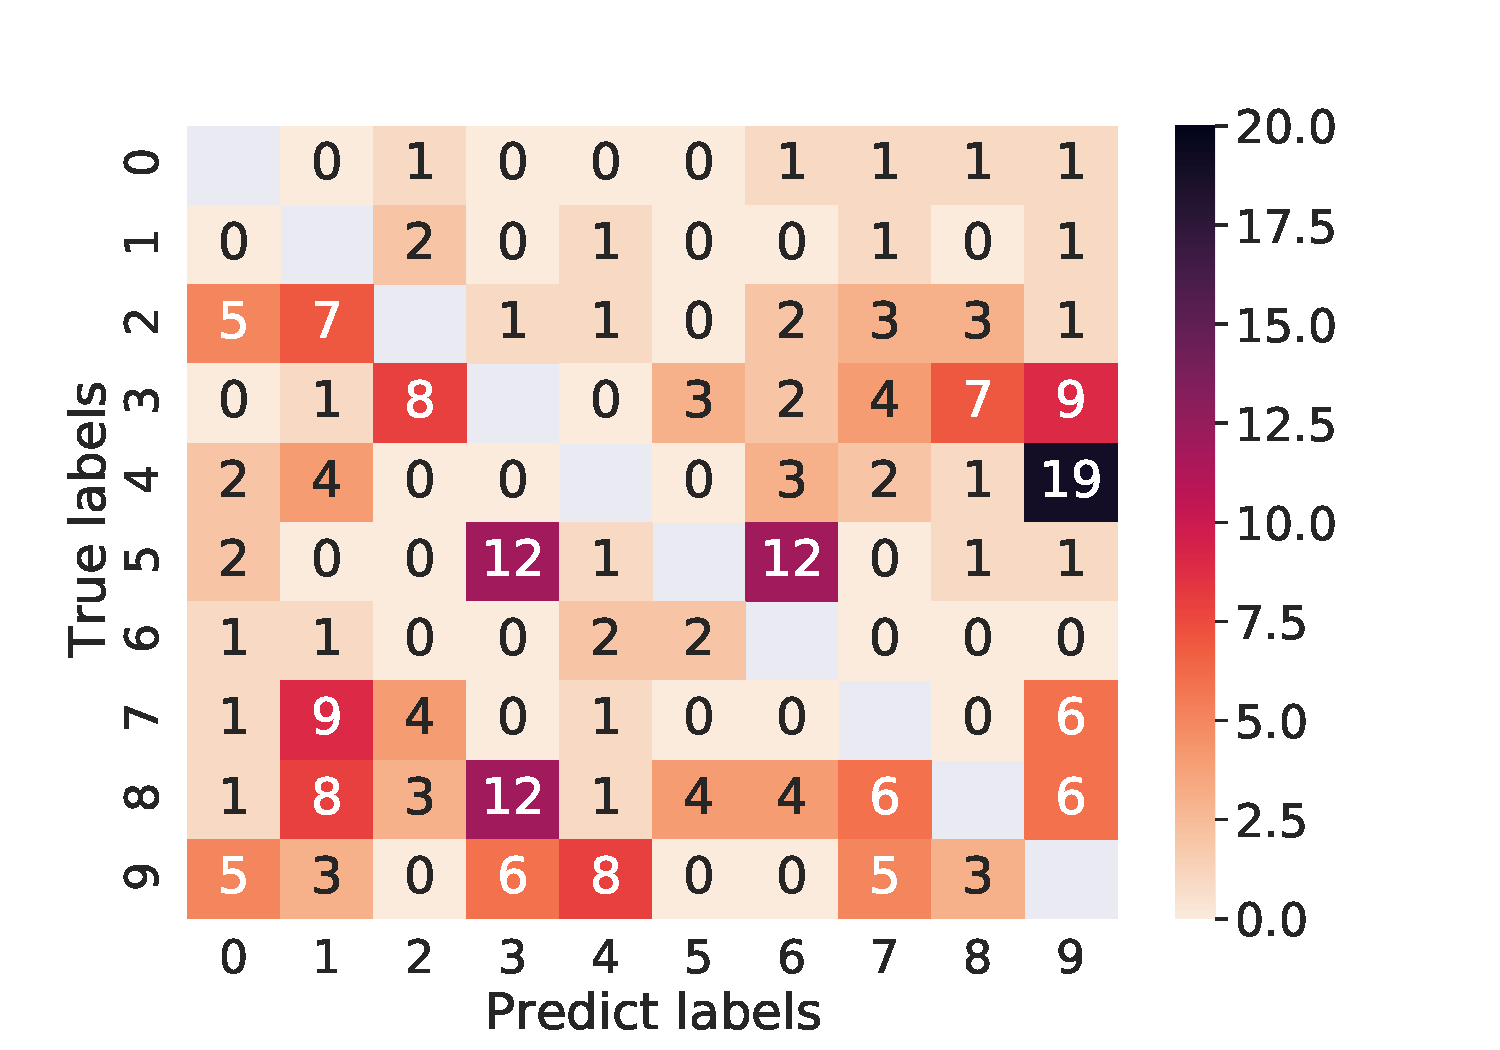
\includegraphics[width=12cm]{task4.pdf}
    \caption{Матрица ошибок}
    \label{pic3}
\end{figure}

Можно выделить самые главные причины ошибок - выбросы и непосредственно ошибки модели. Выбросы в данном случае - это такие объекты, 
которые даже человеку будет тяжело распознать. Эту проблему невозможно исправить никакой моделью. В таблице (Таблица \ref{outlier}) нижже
изображено несколько выбросов.

\newcommand\x{2}
\begin{table}[htb]
    \tabcolsep = -5pt
    \begin{tabular}{lccccccccc}
        \textbf{picture}       & \includegraphics[width=\x cm]{wrong_base/outliers/digit_4_9_7119.pdf}   &\includegraphics[width=\x cm]{wrong_base/outliers/digit_5_3_4400.pdf}  &\includegraphics[width=\x cm]{wrong_base/outliers/digit_5_3_7909.pdf}  &\includegraphics[width=\x cm]{wrong_base/outliers/digit_5_8_1596.pdf}  &\includegraphics[width=\x cm]{wrong_base/outliers/digit_7_1_1214.pdf}  &\includegraphics[width=\x cm]{wrong_base/outliers/digit_8_3_5362.pdf}  &\includegraphics[width=\x cm]{wrong_base/outliers/digit_8_3_8479.pdf}  &\includegraphics[width=\x cm]{wrong_base/outliers/digit_9_0_2025.pdf}  &\includegraphics[width=\x cm]{wrong_base/outliers/digit_9_4_7962.pdf}  \\
        \textbf{true label}    & 4 & 5 & 5 & 5 &7 & 8 & 8 & 9 & 9 \\
        \textbf{predict label} & 9  & 3 & 3 & 8 & 1 & 3 & 3 & 0 & 4 
   
    \end{tabular}
    \caption{Выбросы}
    \label{outlier}
 \end{table}
Рассмотрим ошибки модели. Некоторые из них можно было бы решить аугментацией. Расширив обучающую выборку путем изменения исходных объектов
(поворот, размытие, сдвиг) мы могли бы лучше решать задачу классификации.

В таблице (Таблица \ref{gauss}) изображены несколько обьектов, которые теоретически можно было классифицировать правильно, если бы мы 
применили к ним фильтр Гаусса.
\newcommand\y{3}
\begin{table}[htb]
    \begin{tabular}{lccc}
        \textbf{picture} &\includegraphics[width=\y cm]{wrong_base/gauss/digit_0_6_8798.pdf} & \includegraphics[width=\y cm]{wrong_base/gauss/digit_3_2_3712.pdf} & \includegraphics[width=\y cm]{wrong_base/gauss/digit_8_6_313.pdf} \\
        \textbf{true label} & 0 & 3 & 8 \\
        \textbf{predict label} & 6 & 2 & 6
    \end{tabular}
    \caption{Фильтр Гаусса}
    \label{gauss}
\end{table}

\newpage
В таблице (Таблица \ref{rotate}) изображены объекты, которые были классифицированы неправильно лишь из-за того, что они повернуты
относительно центра изображения слишком сильно. Аугментация могла бы улучшить качество на подобных объектах.
\newcommand\z{3}
\begin{table}[htb]

    \tabcolsep = -6pt
    \begin{tabular}{lcccccc}
        \textbf{picture} &\includegraphics[width=\z cm]{wrong_base/rotate/digit_2_4_385.pdf}  & \includegraphics[width=\z cm]{wrong_base/rotate/digit_2_9_3503.pdf}  & \includegraphics[width=\z cm]{wrong_base/rotate/digit_3_2_2467.pdf}  & \includegraphics[width=\z cm]{wrong_base/rotate/digit_4_1_3715.pdf}  & \includegraphics[width=\z cm]{wrong_base/rotate/digit_4_9_8152.pdf}  & \includegraphics[width=\z cm]{wrong_base/rotate/digit_6_0_6519.pdf}\\
        \textbf{true label} & 2 & 2 & 3 & 4 & 4 & 6 \\
        \textbf{predict label} & 4 & 9 & 2 & 1 & 9 & 0\\
    \end{tabular}
    \caption{Повороты}
    \label{rotate}
\end{table}


\section{Задание №5}
Попробуем улучшить качество нашей модели с помощью аугментации. Подберем по кросс-валидации лучшие 
параметры преобразований изображений среди ниже перечисленных:
\begin{itemize}
    \item rotate deg -- -15, -10, -5, 0, 5, 10, 15
    \item gauss $\sigma$ -- 0.5, 1.0, 1.5
    \item shift px - -3, -2, -1, 0, 1, 2, 3
\end{itemize}

Кроссвалидация проводилась на подвыборке размером 40000.
В результате отобра лучшие параметры получились (см. Таблица \ref{best_param})

\begin{table}[htb]
    \centering
    \begin{tabular}{|l|l|l|l|l|}
    \hline
    $base$  & $rotate, \pm10deg$ & $gauss, \sigma=1$ & $shift\_x, \pm1px$ & $shift\_y ,\pm 1px$ \\ \hline
    0.968 & 0.976          & 0.976       & 0.972      & 0.974   \\ \hline
    \end{tabular}
    \caption{лучшие параметры}
    \label{best_param}
\end{table}

В виду объемности датасета, применим к исходной обучающей выборке Гауссов фильтр и поворот на 10 градусов(можно было взять и -10).
В результате получим обучающую выборку размером 180000.

\newpage
\textbf{Точность на тесте: 0.9835}

Взглянем на матрицу ошибок после агументации(Таблица \ref{conf_matrix_aug}):

\begin{table}[htb]
    \centering
    \tabcolsep = -15pt
    \begin{tabular}{cc}
        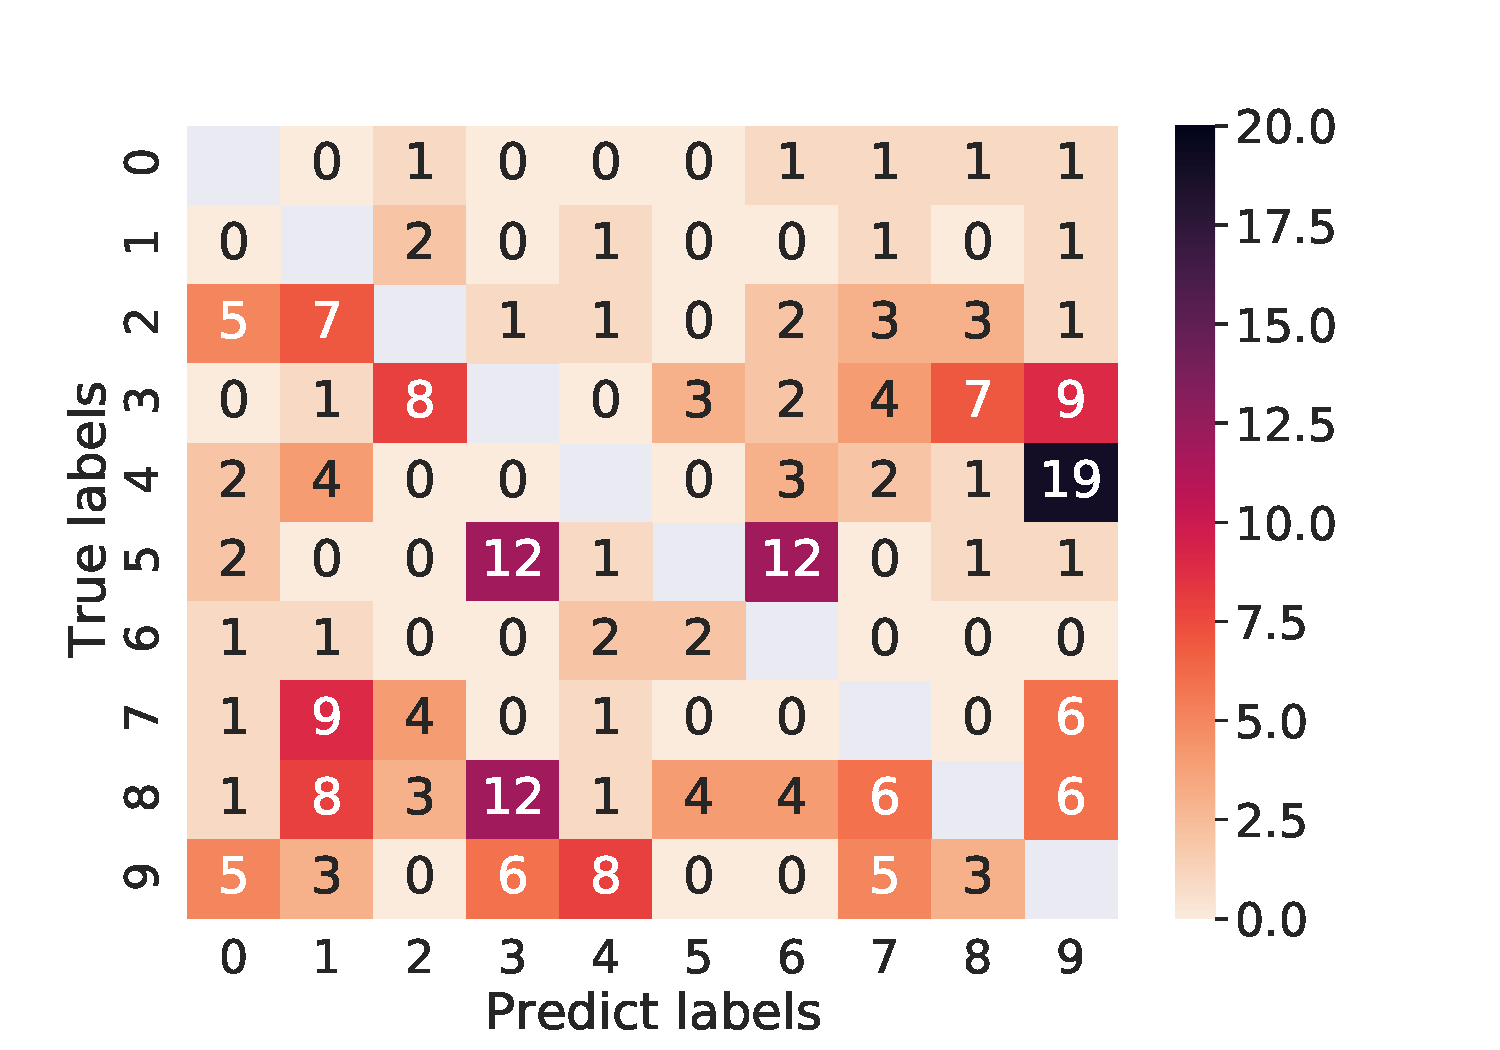
\includegraphics[width=10cm]{task4.pdf} & 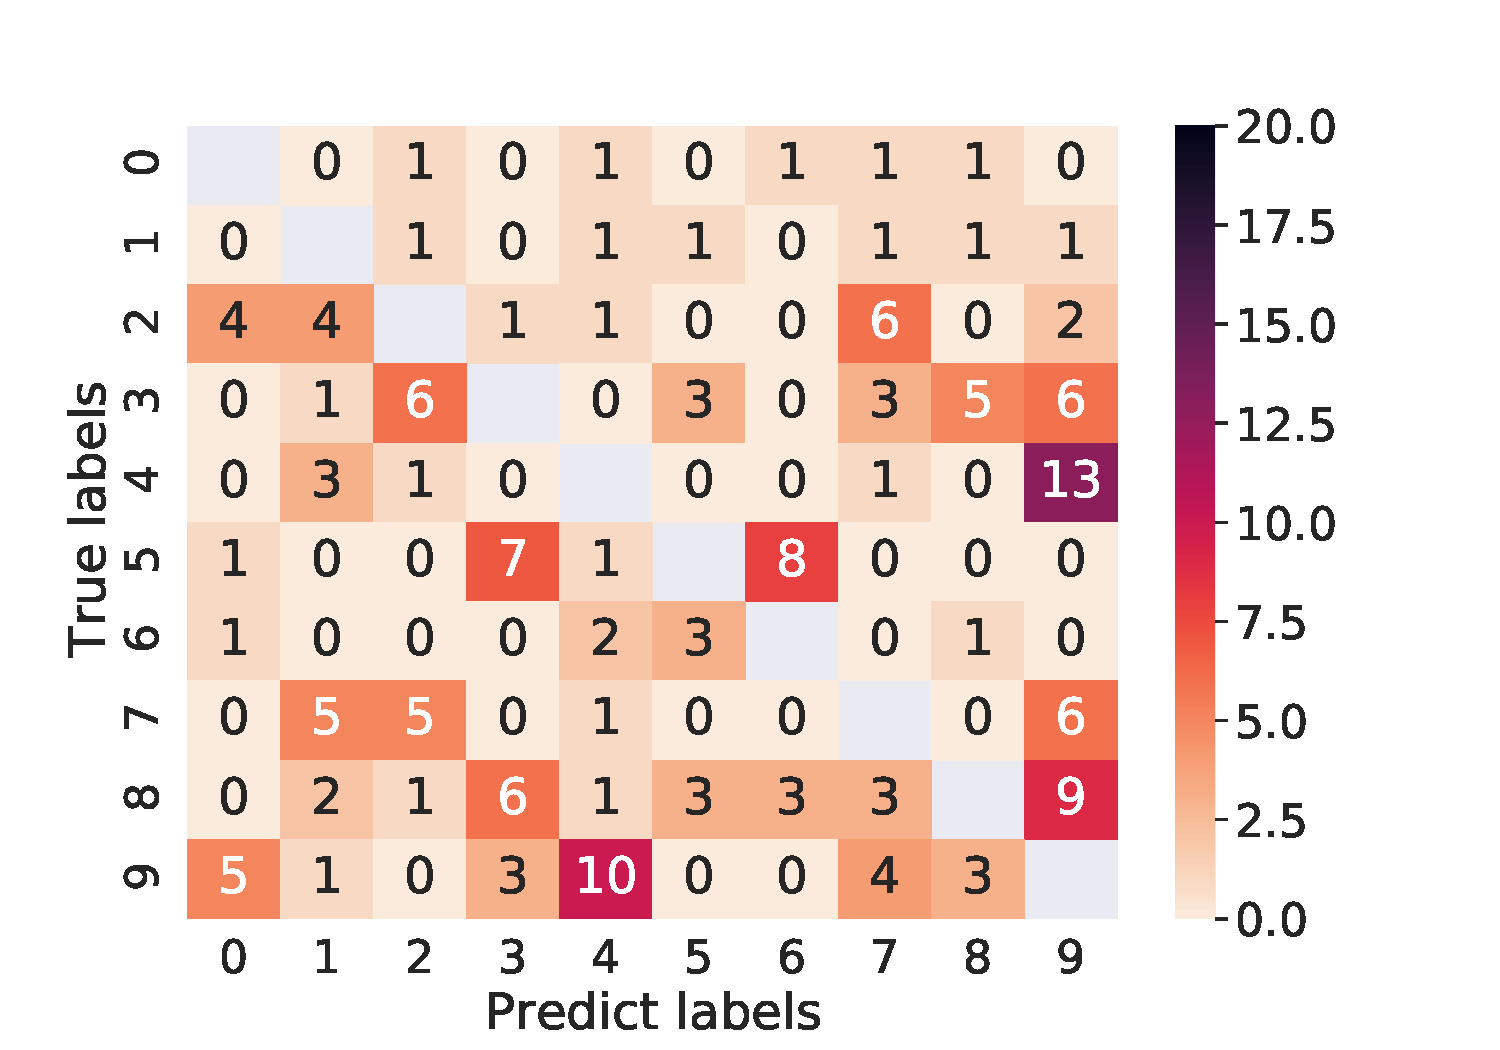
\includegraphics[width=10cm]{task5_conf_mat.pdf}\\
        до агументации & после агументации 
    \end{tabular}
    \caption{Изменение матрицы ошибок после аугментции}
    \label{conf_matrix_aug}
\end{table}

Даже визуально видно, что ошибок стало меньше. Рассмотрим подробнее те объекты, 
на которых справился улучшенный алгоритм, а обычный нет(Таблица \ref{base_vs_aug_obj}):

%\newcommand\x{2}
\begin{table}[htb]
    \tabcolsep = -5pt
    \begin{tabular}{lccccccccc}
        \textbf{picture}       & \includegraphics[width=\x cm]{wrong_base_vs_aug/digit_1_2_5099.pdf}   &\includegraphics[width=\x cm]{wrong_base_vs_aug/digit_2_1_1650.pdf}  &\includegraphics[width=\x cm]{wrong_base_vs_aug/digit_2_4_385.pdf}  &\includegraphics[width=\x cm]{wrong_base_vs_aug/digit_5_6_4233.pdf}  &\includegraphics[width=\x cm]{wrong_base_vs_aug/digit_7_9_9901.pdf}  &\includegraphics[width=\x cm]{wrong_base_vs_aug/digit_8_3_3535.pdf}  &\includegraphics[width=\x cm]{wrong_base_vs_aug/digit_9_4_3297.pdf}  &\includegraphics[width=\x cm]{wrong_base/digit_9_4_5741.pdf}  &\includegraphics[width=\x cm]{wrong_base/digit_9_7_760.pdf}  \\
        \textbf{true label}    & 1 & 2 & 2 & 5 & 7 & 8 & 9 & 9 & 9 \\
        \textbf{predict (base)} & 2  & 1 & 4 & 6 & 9 & 3 & 4 & 4 & 7 
   
    \end{tabular}
    \caption{Объекты, которые удалось правильно классифицировать}
    \label{base_vs_aug_obj}
 \end{table}

Аугментация определенно помогает, увеличить качество, но можно заметить, что на некоторых клетках матрицы ошибок
 значения стали больше. 
В идеале к аугментации нужно подходить более ``умно'', возможно стоило бы размножить объекты из определенного класса или 
научиться понимать в какую сторону лучше повернуть конкретный объект.

\section{Задание №6}
%\begin{thebibliography}{99}
%    \bibitem{deformationmodels}Keysers D. et al. Deformation models for image recognition
%    //IEEE Transactions on Pattern Analysis and Machine Intelligence.
%     – 2007. – Т. 29. – №. 8. – С. 1422-1435.
%\end{thebibliography}

\end{document}